\section{Experiment 3: Influence of Queuing}
This experiment analyzes the performance of TCP Reno and TCP SACK using the queuing algorithms: DropTail and RED. We ran these experiments for the buffer sizes of 100 and 300. When the CBR flow starts at the 4s mark, we see the throughput of the TCP stream start to drop for both RED and DropTail. There is a larger drop in throughput for RED compared to DropTail for both Reno and SACK. The combination of SACK and RED shows the largest drop in throughput. Figure \ref{fig:Queuing_Reno_300} and Figure \ref{fig:Queuing_Sack_300} plot these results for throughput.
\begin{figure}[!htbp]
	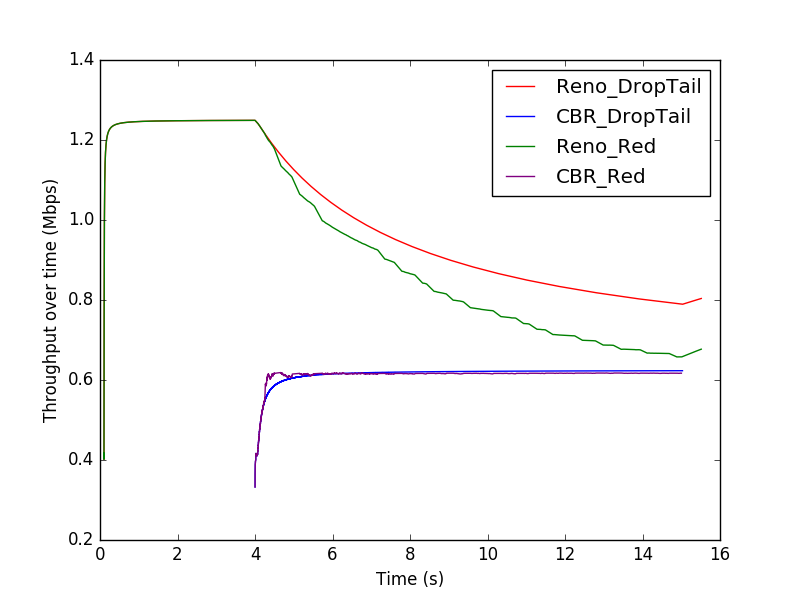
\includegraphics[scale=0.4]{Queuing_Reno_300.png}
	\caption{This graph plots throughput over time between CBR and TCP Reno stream for both RED and DropTail queuing algorithms. The buffer size is held at 300 packets.}
	\label{fig:Queuing_Reno_300}
\end{figure}

\begin{figure}[!htbp]
	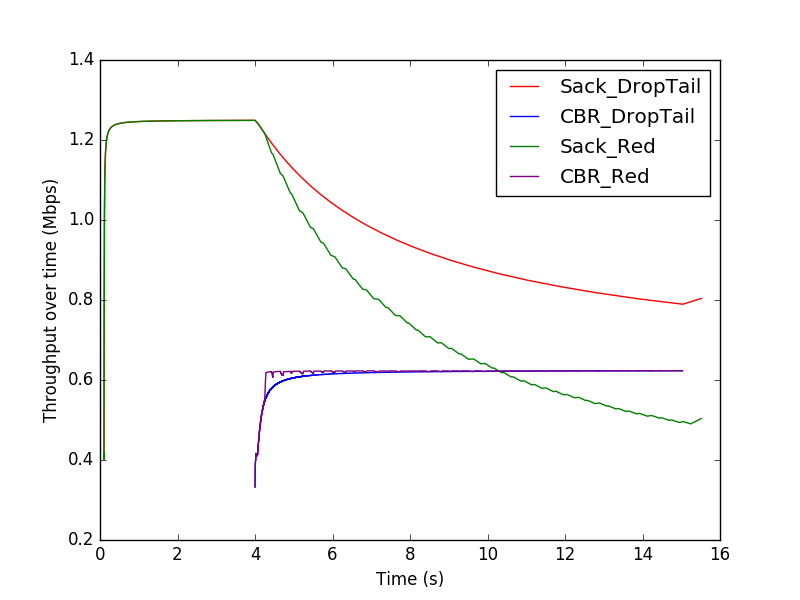
\includegraphics[scale=0.4]{Queuing_Sack_300.png}
	\caption{This graph plots throughput over time between CBR and TCP Sack stream for RED and DropTail queuing algorithms. The buffer size is held at 300 packets.}
	\label{fig:Queuing_Sack_300}
\end{figure}

The low throughput for SACK and RED combination can be explained by the inherent design of these two algorithms. In situations involving multiple packet loss, TCP SACK is aggressive about retransmitting the lost packets. SACK uses partial acks as a signal to wait until all outstanding, or yet to be acknowledged packets are received before coming out of fast recovery. Random Early Detection (RED) accepts all packets when the queue is below some threshhold, and randomly accepts packets when the queue is above the threshhold but still less then the maximum capacity. This allows it to reduce the power of large and fast packet burst which would otherwise monoplize the bandwidth and fill up the queue (in the case of DropTail).  While used in combination with SACK, sending multiple lost packets per RTT results in the retransmitted packets being dropped. In such a scenario, SACK cannot avoid retransmission timeout (RTO). The combination of Reno and RED does slightly better because Reno only has the foresight to keep track of a single lost packet. It can only retransmit one lost packet per window so there is a smaller chance of RTO. 

We also generated plots for end-to-end latency over time and the drop rates (\ref{fig:Queuing_Latency_Sack_100}). After 4s mark, we see that DropTail has larger end-to-end latency and RED reduces the latency. While the latency of DropTail seems to be near constant, the latency of RED fluctuates. The latency of RED is significantly less in comparison to DropTail. However, this reduced latency is coming at a cost of throughput. The result for CBR and Reno was similar. DropTail has higher latency because it fills up the queue, and drops any further packets when the queue is full. Full queue results in larger end-to-end delays. RED on the other hand does not fill up the queue. It uses a threshold value to decide when to drop a packet. If there is congestion, far exceeding the threshold used in RED, packets are randomly dropped.
\begin{figure}[!htbp]
	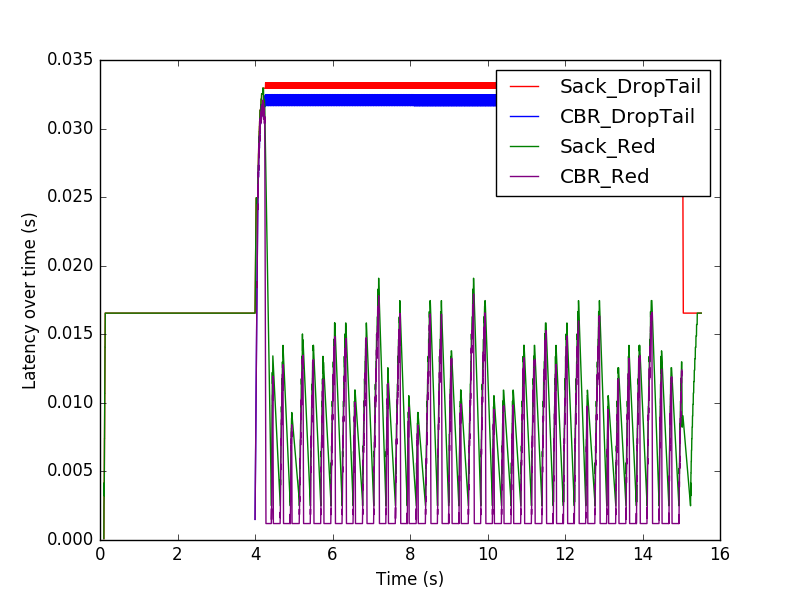
\includegraphics[scale=0.4]{Queuing_Latency_Sack_100.png}
	\caption{The graph shows latency over time for TCP SACK and CBR while using DropTail and RED queuing algorithms.}
	\label{fig:Queuing_Latency_Sack_100}
\end{figure}
How the bandwidth was shared depended on the TCP variant and the queuing algorithm. With DropTail, TCP streams got a larger share of bandwidth compared to CBR which started a little late. Starting both flows at the same instant resulted in more proportionate share of the bandwidth. RED and Reno and RED and SACK lead to a fair share of bandwidth over time.

